\chapter{Defining and Quantifying Failures}
\label{app:risk}

Earlier in \cref{ch:atrds}, a particularly skeptical reader may have noticed several challenges that we did not spend much time discussing, that are inherently tied the stochastic nature of our system. Thus, this chapter will be focused on addressing these challenges, to help us more concretely define failures, and quantify the extent to which we should be concerned about them. We will introduce the concept of risk measures in the univariate case, to first illustrate how we can express our tolerance for risk of failure. Then, we will move on to the more relevant multivariate case, where we discuss some extensions along both the spatial and temporal axes, and will attempt to bridge all of our concepts together under the unifying idea of distortions. Finally, we will end with some brief discussion on how we can account for the network structure of our data in everything we had just outlined.

\section{Guiding Questions}
\label{sec:risk-questions}
For now, let us suppose we have some black-box system, which given an input $z\in \mc Z$, will spit out a value of interest $x=f(z)$, where $x\in \mc X$. We will use this as the canvas for a few guiding questions, to help set the stage for the rest of this chapter.

\paragraph{Why is stochastic harder than deterministic?} We will start with the deterministic case, which would correspond to removing all sources of randomness from our air traffic simulation. Then, if we decide that we have some failure region $\Omega\subseteq \mc X$, we can simply check if the deterministic value $x$ returned by $f$ falls within $\Omega$. However, if $f$ is not deterministic, the question becomes a little more complicated. Instead, for the same input $z$, we could query our system $n$ times and receive $n$ different outputs $x^{(1)},x^{(2)},\ldots, x^{(n)}$, where only some lie in $\Omega$ and the rest do not. Even if we knew the structure of $f$ a priori, we would still have this problem. Furthermore in the black-box case, introducing stochasticity in this manner means that more data is required to understand the shape of $f$, as we can no longer say that a single data point is sufficient.

\paragraph{What exactly is a failure?} Let us be a bit reductive and only consider the case of an arrival time for a single flight, and suppose that the random value $x$ we were discussing now quantifies the delay in minutes. We had previously used 15 minutes, based on federal guidance, as a threshold for delays, so we will consider all values above that to be our failure region. Earlier, one example we had used is considering the probability that $x$ falls above the threshold, or in other words, using the language of catastrophe modeling, the Occurrence Exceedance Probability (OEP). Similarly, we could extend this to multiple occurrences and consider the probability some sort of aggregation, such as average, falls within the failure region. As one might expect, this is known as Aggregate Exceedance Probability (AEP). This sort of solves our problem of converting stochasticity into a more familiar deterministic setting, but is a little inflexible, and perhaps not fully representative of the extent of a failure. Under the exceedance probability framework, or anything similar, we only consider if our samples used to estimate the probabilities lie within the failure region or not, so a delay of 20 minutes would be treated the same as a delay of 200 minutes, even though they are very different. It is possible to vary the threshold and consider all the results, but we might still want to consider an approach that takes the severity of a failure into account more directly. 

\paragraph{How can we specify risk tolerance?} Another weakness with the approach we just discussed is that there isn't really a natural way to specify your tolerance for risk of failure, as we specify the threshold first and then get a probability, instead of the other way around. Naturally, there are so-called risk measures that allow us to do this. For now, let's imagine that we have many samples of delay values in front of us, and that we decide that our tolerance for risk is 5\%. We'll discuss exactly what this means in more detail later. Then, suppose we sort them from smallest to largest, and take the mean of the worst, or largest, 5\% of them. This idea of averaging the worst values is known as the Tail Value at Risk (TVaR). Similarly, we could take the smallest value in that group, in which case we would obtain the Value at Risk (VaR). Then, how does this relate to our questions about failure? First, most related to our previous discussion on exceedance probabilities is the VaR, as it is essentially just the inverse problem of OEP, where we start with the probability, and want to obtain the associated threshold. To check for failure, we could compare this value against a pre-defined threshold for failure. On the other hand, TVaR goes beyond this and also includes some measure of the severity of failures in a region. As we will see later, there plenty of other ways we can go about measuring the risk-aware performance of our system that may be of interest as well.

\paragraph{Is a single number really good enough?} So far, we have only been working with the idea of a single value $x$ that we can use to determine whether or not an event is a failure, and to what extent. However, in real world scenarios, we are often working with multiple variables, which introduces a trade-off between granularity and interpretability. For example, one natural case is considering the delay data at each airport in our network. If we somehow combine all of our information into a single number, then interpretability is achieved, but we may lose some of the granular information in the process. On the other hand, if we maintain full granularity, such as by having a full dimensional vector, then we lose interpretability, as it's much harder to reason about what's going on and more difficult to visualize, compared to fewer numbers. As we will see, it takes some care to express risk associated with inherently multivariate results in an interpretable manner. Also relevant, though less covered in this chapter, is the inherent network structure to our data, which can help guide our decisions here.


\section{Risk Measures}
\label{sec:risk-intro}

Now, we will go further into our guiding questions on defining failures through a quantitative measurement of risk. For now, we will stick to the univariate case, to develop some relevant background before we move on to multiple variables. Here, our goal is to understand how we can bridge the gap between the stochastic and deterministic worlds through risk measures that allow us to collapse probability distributions into values of interest. In this section, we will introduce some background to use in later discussion, from existing literature on risk measures in \cite{Mildenhall_Major_2022, Artzner_Delbaen_Eber_Heath_1999, risks11110194, wirch_hardy_2003}, and so we defer to these sources for a more in-depth development.

\subsection{Preliminaries}

Let $\rx\sim \pxdd$ be a continuous random variable, where $\pxdd$ is the probability density function (PDF) of $\rx$, and with $x\in \mc X$ denoting observations of $\rx$. For simplicity, we will take $\mc X = \RR_{\ge0}$, or the nonnegative reals. We will make the usual regularity assumptions. Additionally, although we will not cover the discrete case, the main idea of the ideas here are roughly the same. Now let $\Fxdd$ and $\Sxdd$ denote the cumulative distribution function (CDF) and survival function (SF) of $\rx$, respectively. Just to review:

\begin{definition}[Cumulative Distribution Function and Survival Function]
    The relationship between the CDF and SF is given by
    \begin{equation}
    \Fxd{x} = \PR{}{\rx\le x} = \int_{0}^x \pxd{t}\,dt = 1-\int_{x}^\infty \pxd{t}\,dt = \PR{}{\rx > x} = \Sxd{x}.
\end{equation}
\end{definition}

We can take analogous definitions for $\ry$ and $y\in\mc Y$. For now, and the rest of this section, we will use these random variables to denote some sort of failure-sensitive quantity, where higher values are worse than lower values. For example, this could be the service time of an airport, or the delay of a flight. 

\paragraph{Risk preferences} First, let us consider the idea of risk preference. Suppose we have $\rx$ and $\ry$, which give us two different distributions of failure-sensitive quantities. Although we have not defined any systematic ways of doing so yet, we might imagine that we have some system to assign a preference to one risk, in this case the $\rx$ and $\ry$, over another. We say that $\rx \succeq \ry$ if $\rx$ is preferred over $\ry$, and vice versa for $\rx \preceq \ry$. It is possible that $\rx\succeq \ry $ and $\rx \preceq \ry$ are both true, in which case $\rx$ and $\ry$ are risk neutral and we do not prefer one over the other. This does not necessarily imply $\rx$ is equal to $\ry$, however. 

\begin{proposition}[Risk preference properties]
    We have three axiomatic properties for risk preferences:
    \begin{enumerate}
        \item \textbf{Completeness}: at least one of $\rx \succeq \ry$ or $\rx\preceq\ry$ is always true.
        \item \textbf{Transitivity}: if $\rx \succeq \ry$ and $\ry\succeq \rz$, then $\rx\succeq \rz$.
        \item \textbf{Monotonicity}: if $\rx \le \ry$ almost surely, then $\rx \succeq \ry$.
    \end{enumerate}
\end{proposition} 
In words, completeness and transitivity just guarantee that we are always able to compare risks in a logically consistent manner. Monotonicity essentially just captures the idea that we should prefer lower values to higher values.

\paragraph{Risk measures} Now we define a risk measure $\rsd$ as a function of a random variable $\rx$, which will help us convert our inherently stochastic quantity into something deterministic that captures both the severity of a potential failure and the associated uncertainty. In doing so, we will also be able to express our risk preference in a systematic manner. In other words, we will be able to quantitatively say what $\rx$ being less risky than $\ry$ means, according to some internal definition of risky. Here, the preference based definition is quite intuitive, and says exactly that:
\begin{equation}
    \rx \succeq \ry \iff \rs{x} \le \rs{y}.
\end{equation}
This formulation also immediately satisfies the first two properties, completeness and transitivity, because of the natural ordering of $\RR$. Monotonicity does not necessarily hold for all choices of $\rsd$, but we will see that it is usually not a problem for the constructions we are interested in. 

\paragraph{Examples} The most obvious example of a useful risk measure is simply the expected value $\rs{\rx}=\EX{}{\rx}$. However, in aggregating the risk distribution in this way, we lose a lot of information about what it looks like, particularly in its variability. Roughly speaking, we should consider risks that are more volatile to be less preferable to risks that are more well behaved and tightly concentrated around the mean. 
\begin{example}[Moment-based Risk Measures]
    Therefore, some risk measures directly attempt to directly penalize this as
    \begin{align}
        \rs{\rx} = \EX{}{\rx} + \lambda\Var\pars*{\rx},\\
        \rs{\rx} = \EX{}{\rx} + \lambda\SD\pars*{\rx},
    \end{align}
    where $\SD\pars*{\rx}=\sqrt{\Var\pars*{\rx}}$ denotes standard deviation, and $\lambda$ is a given constant.
\end{example}

\subsection{Coherence and Convexity}

\paragraph{Risk measure properties} Before we move on, we will introduce a few more useful properties of risk measures.
\begin{itemize}
    \item \textbf{Monotonicity}: if $\rx\le\ry$ almost surely, then $\rs\rx \ge \rs\ry$
    \item \textbf{Sub-additivity}: $\rs{\rx+\ry}\le \rs\rx+\rs\ry$
\end{itemize}
Now, if a risk measure $\rsd$ also satisfies the following two properties, it is also coherent.
\begin{itemize}
    \item \textbf{Positive homogeneity}: $\rs{\alpha\rx}=\alpha\rs\rx$ for $\alpha\ge 0$
    \item \textbf{Translation invariance}: $\rs{\rx+c} = \rs\rx+c$
\end{itemize}
If, instead it only satisfies the following property in addition to the first two, it is convex.
\begin{itemize}
    \item \textbf{Convexity}: $\rs{\lambda\rx+(1-\lambda)\ry}=\lambda \rs\rx+(1-\lambda)\rs\ry$.
\end{itemize}

\subsection{Quantile-based Measures}

\paragraph{Value at Risk} One natural idea is to ask at what level do the worst, say $5\%$, of values start at? We can answer this by simply taking the inverse of the CDF, so that $\Qxd{\pi} = \Fxdinv{\pi}$ and $\Fxd{\Qxd{\pi}} = \pi$. We will note that we are assuming $\Fxdd$ has a well defined inverse for simplicity, but the definition is also similar if that is not the case. With our $5\%$ example, $\pi$ would be $95\%$. As it turns out, this is precisely the Value at Risk (VaR) definition we introduced earlier: we choose some risk level, say $\pi=95\%$, and calculate $\Qxd{\pi}$, which gives us the value where we start to get into the worst $1-\pi=5\%$ of outcomes.

\begin{definition}[Value at Risk]
    The Value at Risk (VaR) risk measure is given by
    \begin{equation}
        \rs{\rx} = \VaR{\pi}{\rx} = \Qxd{\pi}.
    \end{equation}
\end{definition}

The choice of $\pi$ allows you to set your risk tolerance, where higher values of $\pi$ correspond to higher tolerances, and vice versa for lower values. For now, we are using $\pi$ to avoid confusion with the PDF $\pxdd$, but later we may instead just use $p$.

\paragraph{Tail Value at Risk} Often, it also makes sense to capture what the tail actually looks like, instead of a single value from the beginning of the tail. For example, if there is a $4\%$ chance of having a five hour delay and a $96\%$ chance of zero delay, then $\VaRd{95\%}$ would still give you zero delay, even though you might be worried about the non negligible probability of an extremely high delay. To express this, the Tail Value at Risk (TVaR) extends the idea of VaR, but instead calculates the average of the worst outcomes. For a given risk level $\pi$, we have equivalent definitions for this risk measure.

\begin{definition}[Tail Value at Risk]
    The Tail Value at Risk (TVaR) risk measure is given by 
    \begin{align}
        \rs{\rx} = \TVaR{\pi}{\rx} &= \EX{}{\rx \given \rx \ge \VaR{\pi}{\rx} }\\
        &= \frac1{1-\pi}\int_{\VaR{\pi}{\rx}}^\infty t\pxd{t}\,dt\\
        &= \frac1{1-\pi}\int_{\pi}^1 \VaR{s}{\rx}\,ds.
    \end{align}
    Other names for TVaR in the literature are Conditional Value at Risk (CVaR) and Average Value at Risk (AVaR).
\end{definition}
TVaR is also sometimes used interchangeably with Conditional Tail Expectation (CTE) and Worst Conditional Expectation (WCE) for continuous random variables, but these are not equivalent for discrete ones. We will not go into that here, but leave further investigation to the presumably interested reader.

\paragraph{Empirical versions} When we are not given the risk distribution $\pxdd$ in closed form, but are able to generate samples from it, we can estimate the VaR and TVaR as follows.

\begin{example}[Empirical VaR and TVaR \cite{cakmak2020bayesianoptimizationriskmeasures}]
    Suppose we have a sample of $n$ values with order statistics denoted as
    \begin{equation}
        x_{(1)} \le x_{(2)} \le \cdots\le  x_{(n)},
    \end{equation}
    then the empirical VaR and TVaR at risk level $\pi$ are given by the analogous
    \begin{align}
        \eVaR{\pi}{\rx} &= x_{(m)} \\
        \eTVaR{\pi}{\rx} &= \tfrac{1}{n - m+1}\sum_{i=m}^{n} x_{(i)} ,
    \end{align}
    for $m=\lceil \pi\cdot n\rceil$, where $\lceil\cdot\rceil$ is the ceiling function.
\end{example}

This sort of Monte Carlo integration is also applicable to other risk measures that we will see later, but we will not be discussing it in depth.

\subsection{Distortion Functions}

Notice that VaR and TVaR still have something in common with just taking the expected value. Namely, we are still essentially taking a weighted average of the possible outcomes, it's just that in the expected value case, we just use a weighting given by our density $\pxdd$, whereas VaR and TVaR will distort the density in some way to express our risk preference. VaR places full weight on a single point, while TVaR redistributes the weight across the tail beyond a point. This motivates the introduction of so-called distortion functions, which are defined as follows.

\begin{definition}[Distortion Function]
    An increasing $g:[0,1]\to[0,1]$ is a distortion function if $g(0)=0$, $g(1)=1$, and $g(s)\ge s$ for all $0\le s\le 1$. 
\end{definition}

Often, $g$ is taken to be concave to provide some convenient properties, and so we will assume this to be part of the definition for the rest of our development. 

\subsection{Spectral Risk Measures}

Now, we can see how these distortion functions can be used to generate risk measures with useful properties under a single unifying framework.

\begin{definition}[Spectral Risk Measure]
    The spectral risk measure (SRM) associated with a distortion function $g$ is given by 
    \begin{equation}
        \rs{\rx}=\int_0^\infty g(\Sxd{t})\,dt = \int_0^\infty tg'(\Sxd{t})\,d\Fxd{t} = \EX{}{\rx g'(\Sxd{\rx})},
    \end{equation}
    assuming the reasonable tail decay condition $tg(\Sxd{t}) \to 0$ as $t\to\infty$.
\end{definition}

Unlike VaR and TVaR, an empirical estimation is a bit more involved, but still possible, though we will not go into that now\cite{pandey2019estimationspectralriskmeasures}. Here is an alternative definition that more directly illustrates the re-weighting process.

\begin{definition}[SRM via Spectral Weight Function]
    An equivalent definition for our spectral risk measure is as follows:
    \begin{equation}
        \rs{\rx} = \int_0^1 q(p) g'(1-p)\,dp = \int_0^1 q(p)\phi(p)\,dp ,
    \end{equation}
    where $p = \Fxd{t}$ and $t=q(p)=\VaR{p}{\rx}$, so that $d\Fxd{t} = dp$. 
\end{definition}

Here, $\phi(p) = g'(1-p)$ is referred to as the spectral weight function, as it describes how much weight our spectral risk measure places on the outcome $q(p)=\VaR{p}{\rx}$. Then, as described earlier, we have the following:

\begin{example}[SRM Formulation of VaR]
    Consider the distortion function $g(s) = \mbm{1}_{s>1-p}$, or the step function that is $0$ for $s<1-p$ and $1$ for $s\ge p$. Then $g'(s)=\delta(1-p)$, where $\delta(\cdot)$ is the Dirac delta function, and so $\phi(s) = g'(1-s) = \delta(p)$. Therefore, we have
    \begin{equation}
        \rs{\rx} = \int_0^1 \VaR{p}{\rx}\cdot \delta(p)\,dp = \VaR{p}{\rx}.
    \end{equation}
\end{example}

\begin{example}[SRM Formulation of TVaR]
    Consider the distortion function $g(s) = \min(\tfrac{s}{1-p},1)$. Then $g'(s)$ is equal to $\tfrac1{1-p}$ for $s\le 1-p$ and is zero otherwise, so
    \begin{equation}
        \phi(s) = g'(1-s) = \begin{cases}
            \frac1{1-p} & s\ge p \\
            0 & s< p,
        \end{cases}
    \end{equation}
    and applying this weighting in our integral yields
    \begin{equation}
        \rs{\rx} = \int_{p}^1 \VaR{p}{\rx}\cdot \frac1{1-p}  = \TVaR{p}{\rx}.
    \end{equation}
\end{example}

For the remainder of this section, we will not focus too much on the technical details of developing distortion functions and spectral risk measures. Instead, we will mainly work with SRMs at a high-level, interpreting them as a principled re-weighting of outcomes according to a user's risk preference. To this end, the previously given examples of VaR and TVaR will be helpful to keep in mind.


\section{Multivariate Extensions}
\label{sec:risk-multi}

So far, we have mostly been discussing risk regarding a single random variable $\rx$. However, in our air traffic problem, we actually have multiple different axes on which individual risks, such as flight delays, are naturally divided along. While there is related work in generalizing univariate risk measures to the multivariate case, such as in \cite{Shushi_Yao_2020} and \cite{RePEc:hal:wpaper:hal-01831481}, we will consider those details outside of our scope for now, and instead focus on the main ideas behind extending to the multivariate case.

\paragraph{Spatial axis} The first is due to the inherent network structure of the problem. Let us forget about temporal considerations for a moment, and pretend that we have a single value for each airport, such as mean delay per node, that represents their individual risk. Naturally, we know that these are all correlated. Now suppose we tried to naively reduce our problem to the univariate case by aggregating all of our delays together into a single mean delay for the whole network. One benefit is that we improve interpretability, as a single number is much easier to understand than many, especially in our case where we may have thousands of different airports. However, by combining all of our granular information in this way, we destroy the inherent network structure to our data. Additionally, not all delays are created equal, and our risk tolerance may be different for certain nodes or sections of the overall network based on our prior beliefs about each specific airport. However, including the full granularity of the data is perhaps not the right answer either.

\paragraph{Temporal axis} The second is due to the inherent temporal structure of the problem. Focusing on a single airport for a moment, it is possible that our delays vary depending on time of day, as the data comes from a time varying process. For example, one common phenomenon is that less delay may be observed in the beginning of the day, but it steadily increases for flights later in the day as delays propagate throughout the network. Then, as we can see, simply taking a mean may not be fully representative of the data, as a day with a constant moderate delay of 15 minutes is very different from a day with spikes of 150 minute delays occurring 10\% of the time. Maintaining full granularity, we could take this to be a vector containing the full delay profile of this particular node for the day, which may include hundreds of flights. Once again, we reach the question of how we can meaningfully collapse this into a more interpretable representation.

\subsection{Dimensionality}

For now, we will return to the simplified case for the spatial axis, and return to the temporal axis later. For this setup, let us suppose we have a network $G$ with vertex and edge sets $V$, $E$, respectively. Enumerate the vertices in $V$ as $v_1,v_2,\ldots,v_n$, and include an edge $e_{i,j}$ in $E$ if an edge exists between $v_i$ and $v_j$. Then, similarly to before, equip each node $v_i$ with random variable $\rx_i$ which we will use to analyze the risk of each node and the network as a whole.

\paragraph{Univariate aggregation} First, we will compare some methods to aggregate these risks into a single risk or value. These will be easier to use, but perhaps more restrictive than our later inherently multivariate discussions. However, since univariate is just a special case of multivariate, it will still be useful to motivate our main ideas here.

\paragraph{Weighted average} One way to do so is by taking a weighted average of our existing risks.

\begin{example}[Weighted Average Aggregation]
    Let $w_i$ be an importance weight placed on node $v_i$. Then, we can define a network risk
    \begin{equation}
        \rx = \frac{\sum_{i=1}^n w_i \rx_i} {\sum_{i=1}^n w_i}.
    \end{equation}
\end{example}

We can choose the weights $w_i$ in various ways. For example, if the $w_i$ are simply chosen to be the number of flights that have an endpoint at node $v_i$, and the original $\rx_i$ are the mean flight delays for each node, then this $\rx$ is essentially just a straight average of all flight delays across the network. It may also make sense to place heavier weight on more important nodes. For example, in a hub and spoke network structure, delays at a central hub may be of greater interest. However, notice that this aggregation transformation does not preserve risk measures, so it is not guaranteed that 
\begin{equation}
    \rs{\rx} = \frac{\sum_{i=1}^n w_i \rs{\rx_i}} {\sum_{i=1}^n w_i}
\end{equation}
also holds, as not all risk measures have the linearity property like expected value does. In fact, if we choose an SRM for $\rho$ with a concave distortion function, then it is coherent and therefore subadditive, so we could only say
\begin{equation}
    \rs{\rx} \le \frac{\sum_{i=1}^n w_i \rs{\rx_i}} {\sum_{i=1}^n w_i}
\end{equation}
Then, how can we robustly combine information from each of the individual risk measures without having to work with an aggregated risk, which may be more difficult to analyze?

\paragraph{Node-level distortions} Let us first consider a simple example, where we choose $\TVaRd{p}$ as our risk measure, and apply it to each node as $\TVaR{p_i}{\rx_i}$. Then, a simple way to express our risk preference on a node level is to vary the risk level $p_i$. Nodes that are considered to be more critical should use a higher $p_i$ to distort their distributions more toward the right tail, while those that are less critical can set their level at lower values. Note that at risk level of zero, the TVaR and expected value are equivalent. However, our risk measures are still inherently decoupled with this structure, and we would still need to combine them once again after the fact somehow. It is then clear that this pattern of aggregation will always have limitations if we want to reduce dimension this aggressively. However, with this node-level approach, we can maintain slightly better expressivity compared to before, because of the more interpretable method of setting risk tolerance levels instead of having to choose weights without as direct of an interpretation. To generalize this slightly, we can work directly with distortions.

\begin{example}[Node-level distortions]
    Select distortion functions $g_i$ with associated SRM $\rho_i$ for each node. Then, compute each $r_i = \rsg{i}{\rx_i}$, and aggregate results into a single 
    \begin{equation}
    r = \rho^*(\rx_1,\ldots,\rx_n) = \frac{\sum_{i=1}^n w_i \rsg{i}{\rx_i}} {\sum_{i=1}^n w_i} = \frac{\sum_{i=1}^n w_i r_i} {\sum_{i=1}^n w_i}
    \end{equation}
\end{example}

\paragraph{General pattern} In the two examples above, we can see some steps that occur in different orders. One is applying an aggregation function, say $g(\cdot)$, that takes care of the dimensionality reduction goal. This could be a weighted average, as we saw before, or some other function, such as the maximum function. The choice of aggregation function is somewhere risk preference can be expressed. For example, choosing to use an average represents a greater risk tolerance than maximum, which represents a lower risk tolerance more focused on the worst-case outcomes. Another step is applying a risk measure $\rho$, and the order of these steps is not interchangeable. As we saw earlier, any useful risk measure should have some parameter built in to express risk preference as well. 

Note that just because we are hoping to end up with a univariate value does not preclude viewing our risks in an inherently multivariate way. For example, one way we could consider aggregation is by $n$-dimensional balls centered at the origin. Depending on the choice of metric used to define said balls, we can obtain the interpretations we described above.


\subsection{Network Considerations}

\paragraph{Multivariate expression} We can now generalize a little bit and focus on how we might represent our collection of risks in as a multivariate value, noting that this is a generalization because we are still trying to reduce dimensionality, just not necessarily to a single dimension. For now, we will work generally and defer how we might want to use knowledge of the network structure to later. One initial step could be to identify a subset of existing nodes that represent the network in some useful way, for example, by taking the busiest airports in the network, and calculating risk metrics individually. This is a similar idea to selecting weights that we discussed earlier, where we now attempt to extract a sparse representation by setting enough of the node weights to zero. If we already know some risks are correlated, such as nearby airports that perform similarly to each other, it can also make sense to combine them for analysis. If we do not know any of this, another approach is to combine nodes from spatially similar regions.

\paragraph{Spatial distortions} We can consider this idea of selecting or weighting nodes spatially as a sort of spatial distortion of the risks within our network. Similarly to when we defined spectral risk measures through a distorted analogue of expected value, we can also define a distortion on the spatial structure of our network as a re-weighting of either the risks themselves of the risk tolerances. We will see what this means in more detail later. For now, the main idea is just that when we are applying distortions to generate risk measures, we distort our risks to emphasize the outcomes that are of more interest to us, such as with TVaR and the typical tail behavior. Similarly, when we are more interested in a particular area of the network, we are also applying a different sort of distortion, but altogether, all we are doing is taking the typical behavior of the overall network, distorting it in various ways, and working with a risk-adjusted version of the model, based on our specified risk preference.

\paragraph{Swapping edges and nodes} So far, we have taken a rather node-centric view of the problem. However, it is also natural to consider the problem from the perspective of edges, as we may be just as interested about what happens along specific routes as what happens at specific airports. To reuse any tools we may develop for the latter case in the former, we can generate the medial graph $H$ of our network $G$. This is done by initializing a node for each edge in the original graph, and connecting two of these new nodes in $H$ if their corresponding edges in $G$ shared a vertex.

\subsection{Temporal Considerations}

Now we will turn our attention to the temporal aspect once again, or in other words, how we might come up with definitions for these $\rx_i$ variables at each node. For now, we will use the example of flight delays to align with our work in \cref{ch:atrds}, but we can use similar methods for other metrics as well.

\begin{example}[Flight Delays]
    Let $\rx_i^{(1)}, \rx_i^{(2)}, \ldots, \rx_i^{(n)}$ be a sequence of delays recorded for $n$ flights in chronological order at node $v_i$ on a given day. Then, let $h_i$ be some temporal aggregation function such that \[\rx_i = h_i\pars*{\rx_i^{(1)},\rx_i^{(2)}, \ldots, \rx_i^{(n)}}.\]
\end{example}
This is not the only way we can collapse the temporal axis, so to speak, but we will focus on this for now to fit in with our previous spatial discussion.

\paragraph{Temporal distortions} Similarly to before, we might be more interested in a particular region of our temporal data. This time, instead of placing greater weight on one portion of the overall network, we might want to focus on one particular region, such as the later part of the day, as that might be more representative of how delays build up. Alternatively, we may want to analyze the accumulation of delay at a particular node, and so instead might want to adjust delays for when in the day they were from to offset the propagated delays effect. Practically speaking, this could be attempting to fit a least squares model to the data, and using the slope as a metric of how quickly delay accumulated. This also introduces another idea: not only might we be interested in a specific area of our risks, whether that be well-defined or not, we might also be interested in the marginal changes as our risk develops along a particular axis. 

\paragraph{Time-agnostic aggregation} Note that incorporating the temporal aspect of our data does require that we make some assumptions or have some existing knowledge about that particular relationship, in order for it to be useful. Similarly to the spatial case, we can still fall back on less informed methods if we do not have this information available, or do not want to make assumptions. Some natural choices would be to compute a statistic that appears to adequately represent the data, such as the mean. If we wanted to go further, we could treat each of the observations $x_i^{(j)}$ as samples from the random variable $\rx_i$, and estimate a sufficiently interesting risk measure from these, such as the empirical TVaR we introduced earlier, if we wanted to capture a measure of the worst set of values. Not all methods need to lie in only one of these categories. For example, we might take temporal structure into account by breaking up our observations into groups based on hour, and then apply a time-agnostic aggregation by taking the worst average out of all of these groups.


\subsection{Distortion Framework}

Before we move on, we will take a minute to put everything we just talked about together. So far, there are three axes along which to incorporate our risk preferences that we have discussed so far. The first is a general notion of risk measures by applying a distortion to a probability distribution. The second is the spatial aspect, where we may decide to distort our view toward certain areas of our network, and the third is the temporal aspect, where we do the same except applied based on time of event rather than location. In addition to these, we also have a notion of aggregation that we must include, which is meant to collapse our data down into something more interpretable for use in assessing risk. Notably, all of these steps do not need to be applied in any particular order, as we saw earlier. What we have not yet discussed in depth is how to extend these ideas to incorporate information that is based within the network structure of our data.


\section{Connections to Electrical Networks}

In this final section, we will attempt to draw some simple potential connections between the network-based model of risks we previously introduced, and the rich field of random walks on graphs and electrical networks, in the hopes that there may be tools that are of use to us here. There will not be much in the way of results in this section, as it will mostly be a series of loosely connected ideas that are aimed at helping us use network-based knowledge in our earlier development. There is some related work in bridging the gap between methods for analyzing networks and aviation data. For example, \cite{Li_Gopalakrishnan_Pantoja_Balakrishnan_2021} applies graph signal processing techniques to characterize the spatial distribution of delays in a network, and \cite{Huynh_Ng_Toh_Feng_2024} studies connections between network measures of nodes and passenger volumes using various parametric and non-parametric models. However, this section is only meant to briefly draw some initial connections to the previous development of risk measures, and so we will be deferring a more in depth study to later work.

\subsection{Preliminaries}

As before, we consider a connected graph $G=(V,E)$. This time, we will also consider an corresponding representation where each undirected edge $e$ is replaced with two directed edges $e^\rightarrow$ and $e^\leftarrow$. We will refer to the set of directed edges as $E^\rightarrow$, and say that an directed edge $e$ goes from node $e^-\to e^+$. We will also let $E^\rightarrow_v$ denote the set of edges $e$ for which $e^-=v$. Now endow the graph with conductances $c(e)$ for each edge $e$, where $c:E\to\RR^+$, and define the resistance to be the reciprocal $r(e) = c(e)^{-1}$. We can also define the conductance of a vertex as $c(v) = \sum_{e\in E^\rightarrow_v} c(e)$. While this model has a direct relationship to electrical networks in the physical sense, we will mainly be considering the network structure \cite{lyons2017probability}.

\subsection{Spatial Distortions}

With this machinery, we can generate one possible formulation of spatial distortions, to formalize some of the ideas discussed earlier. Note that our discussion of temporal distortions worked similarly to the usual case, so we will not be going further into that. For this problem setting, we will first choose a region of interest, as a subgraph induced by nodes $W=\{v_1,v_2,\ldots,v_m\}$. Then, we will define a way to grow outward from this region. 

\begin{definition}[Graph Distance]
    Let $d(u,v)$ denote the graph distance, or minimum number of edges along any path between $u$ and $v$ in $G$. Then, we can also define the ball of radius $r$ centered at $v$ as
    \begin{equation}
        B_v(r) = \{u \mid d(v,u) \le r\}.
    \end{equation}
\end{definition}

We can define an analogous notion of distance to a set $W$ as the minimum distance to any $v\in S$, and use that to define a ball centered at $W$. Then, we can define the analogue of a survival function as 
\begin{equation}
    S(d) = \frac1Z\sum_{i>d}\sum_{v\in B_W(i)} c(v),
\end{equation}
where $Z=\sum_{v\in V}c(v)$ is a normalizing constant. Note that $S(d)$ essentially corresponds to behavior at the boundary of a shell at distance $d$ away from our reference set $W$. Now, as before, we can take a distortion function $g:[0,1]\to[0,1]$, and compute $g'(S(d))$ for each $d$, and we now have a re-weighting that we can apply to our conductances along each shell to express the preferences encoded within the distortion. We can perform a similar process, but with separate uninformed weights instead of the assigned conductances as well.


\subsection{Gradients and Divergences}

First, we will need to introduce the idea of calculus on graphs, which we will use throughout. Since our main focus so far has been using network structure to help us inform importance weightings, we will first need to understand how to analyze functions that place weights on nodes and edges. For now, assume all unit conductances $c(e)\equiv 1$.

\begin{definition}[Gradient of a Node Function \cite{hutchcroft2022notes}]
    Suppose we have a function $F:V\to \RR$, then define the gradient of $F$ to be
    \begin{equation}
        \nabla\cdot F(e) = c(e)\cdot\pars*{F(e^+)-F(e^-)}.
    \end{equation}
    %Note that $\nabla\cdot F(e^\rightarrow) = -\nabla\cdot F(e^\leftarrow)$. We call an edge function with this property of negation upon edge direction reversal a 1-form. For now, take $c(e)\equiv 1$.
\end{definition}

\begin{definition}[Divergence of an Edge Function \cite{hutchcroft2022notes}]
    Suppose we have a function $f:E^\rightarrow\to\RR$, then define the divergence of $F$ to be 
    \begin{equation}
        \nabla\cdot f(v) = \sum_{e\in E^\rightarrow_v} f(e).
    \end{equation}
\end{definition}

Now let us consider a simple and interpretable edge function, where we simply place the scheduled number of flights along a route as the edge function $f$. For now, make the simplifying assumption that the flows of aircraft are balanced, so that along each route there are the same number of flights going each way. Then the divergence $\nabla\cdot f(v)$ is essentially the number of flights scheduled to depart from a node during a given day, which is the precisely the same as the volume weighting definition from earlier sections. Similarly, we could define the node function $F$ as the number of flights scheduled to depart from a node during a given day, and obtain an analogous volume weighting for edges using $\nabla\cdot F(e)$.

As we can see, these notions are useful because they allow us to map our node-based information to edge-based information, and vice versa. This is potentially relevant because not all information that can be used to augment the network may be as easily understood in both forms.

\subsection{Note on Exhaustions}

Exhaustions are a tool to take infinite volume limits of networks, by considering progressively larger subnetworks $G_n=(V_n,E_n)$ that approach the full network $G=(V,E)$. While not immediately relevant for us, as our network of interest must be finite, there is a particular detail regarding how to handle the boundary of a subgraph that is important to consider.

\begin{figure}[htb!]
    \centering
    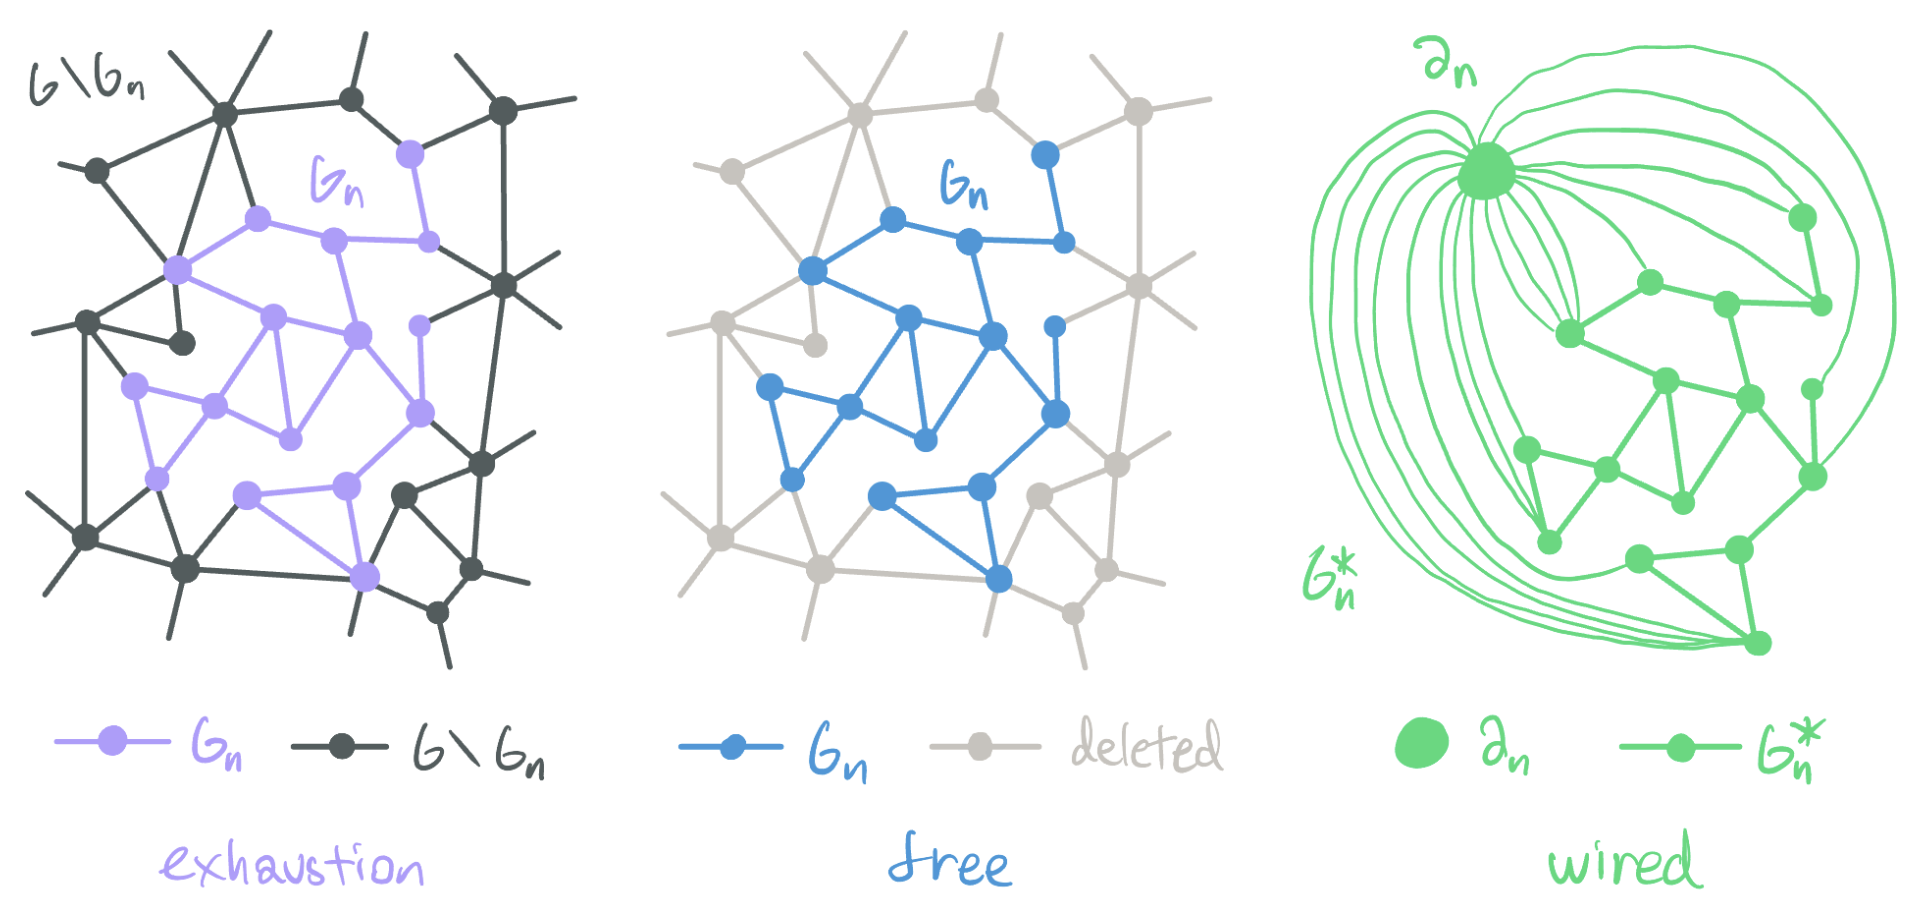
\includegraphics[width=.9\linewidth]{media/exhaustions.png}
    \caption{An illustration of the differences between the free and wired exhaustions. On the left, a subgraph (purple) is shown among a portion of an infinite graph $G$ (black). In the center, the corresponding free exhaustion $G_n$ (blue) is shown among the deleted parts of $G$ (grey). On the right, the corresponding wired exhaustion $G_n^*$ and its wired supernode $\partial_n$ are shown (green).}
    \label{fig:exhaustions}
\end{figure}

\paragraph{Free and wired exhaustions} At a particular step in the exhaustion, when we have vertex set $V_n\subseteq V$, there are two ways we can handle the rest of the graph that is not included in the subgraph $G_n$ induced by $V_n$. The first method is known as the free exhaustion, where all of $G\setminus G_n$ is deleted. The second is known as the wired exhaustion, because all of $G\setminus G_n$ is ``wired" together with the resulting self loops deleted, into a single supernode $\partial_n$. The key difference is that free exhaustions essentially destroy the boundary, because of the deletion of everything outside $G_n$, while wired exhaustions preserve the boundary edges in the form of connections to $\partial_n$ \cite{Benjamini_Lyons_Peres_Schramm_2001}.

\paragraph{Why does this matter?} Note that our study in \cref{ch:atrds} is essentially a rather degenerate case of this idea, as we only had a single node, and thus our subgraph was essentially just the single node. However, we incorporated the boundary information by way of including all incoming and outgoing flights. In this sense, the wired version was far more representative than the free version, because otherwise we would have just had nothing going on at our single node. Although most cases will not be as extreme, and even though there are reasons for going with the free method, such as simplifying the model, boundary behavior is an important consideration that we must make if we are going to be distorting our network to primarily focus on certain areas.

\section{Summary}

In this chapter, we first introduced some relevant background to help us define failures and quantify their potential severity in the stochastic setting. We covered risk preferences, then a basic formulation of risk measures, and their associated properties. Then, we covered closed-form and empirical versions of two commonly used quantile-based risk measures, VaR and TVaR, and used them to motivate the idea of distortion functions. We then covered distortion functions as a way to define spectral risk measures to generalize some of the ideas we had previously introduced. After all this, we moved on to multivariate extensions, and discussed different ways of dealing with the spatial and temporal axes. We also discussed a pattern of combining aggregation and distortion in the context of dimensionality reduction of high dimensional risk measure values. Finally, we drew some connections between those ideas and electrical networks, to motivate potential areas for future work.